


\begin{landscape}
\begin{figure}[htb]\begin{center}
\vskip-1.5cm
\hskip-2cm
\resizebox{1.5\textwidth}{!}{
	\subfigure[]{
  	\includegraphics[width=0.3\textwidth]{appendices/figures/htx_control_unscaled/LepPt_MUON_4jetex0btagex_NOMINAL.eps}}
	\subfigure[]{
  	\includegraphics[width=0.3\textwidth]{appendices/figures/htx_control_unscaled/MET_MUON_4jetex0btagex_NOMINAL.eps}}
	\subfigure[]{
  	\includegraphics[width=0.3\textwidth]{appendices/figures/htx_control_unscaled/JetPt1_MUON_4jetex0btagex_NOMINAL.eps}}
	\subfigure[]{
  	\includegraphics[width=0.3\textwidth]{appendices/figures/htx_control_unscaled/HTHad_MUON_4jetex0btagex_NOMINAL.eps}}
	\subfigure[]{
  	\includegraphics[width=0.3\textwidth]{appendices/figures/htx_control_unscaled/HTAll_MUON_4jetex0btagex_NOMINAL.eps}}
}\\
\hskip-2cm
\resizebox{1.5\textwidth}{!}{
	\subfigure[]{
  	\includegraphics[width=0.3\textwidth]{appendices/figures/htx_control_unscaled/LepPt_MUON_5jetex0btagex_NOMINAL.eps}}
	\subfigure[]{
  	\includegraphics[width=0.3\textwidth]{appendices/figures/htx_control_unscaled/MET_MUON_5jetex0btagex_NOMINAL.eps}}
	\subfigure[]{
  	\includegraphics[width=0.3\textwidth]{appendices/figures/htx_control_unscaled/JetPt1_MUON_5jetex0btagex_NOMINAL.eps}}
	\subfigure[]{
  	\includegraphics[width=0.3\textwidth]{appendices/figures/htx_control_unscaled/HTHad_MUON_5jetex0btagex_NOMINAL.eps}}
	\subfigure[]{
  	\includegraphics[width=0.3\textwidth]{appendices/figures/htx_control_unscaled/HTAll_MUON_5jetex0btagex_NOMINAL.eps}}
}\\
\hskip-2cm
\resizebox{1.5\textwidth}{!}{
	\subfigure[]{
  	\includegraphics[width=0.3\textwidth]{appendices/figures/htx_control_unscaled/LepPt_MUON_6jetin0btagex_NOMINAL.eps}}
	\subfigure[]{
  	\includegraphics[width=0.3\textwidth]{appendices/figures/htx_control_unscaled/MET_MUON_6jetin0btagex_NOMINAL.eps}}
	\subfigure[]{
  	\includegraphics[width=0.3\textwidth]{appendices/figures/htx_control_unscaled/JetPt1_MUON_6jetin0btagex_NOMINAL.eps}}
	\subfigure[]{
  	\includegraphics[width=0.3\textwidth]{appendices/figures/htx_control_unscaled/HTHad_MUON_6jetin0btagex_NOMINAL.eps}}
	\subfigure[]{
  	\includegraphics[width=0.3\textwidth]{appendices/figures/htx_control_unscaled/HTAll_MUON_6jetin0btagex_NOMINAL.eps}}
}
	\caption{Comparison between data and prediction in the $e$+jets channel in the control samples
          with $=4$ jets (a--e), $=5$ jets (f--j), $\geq 4$ jets (k--o),  and $=0$ $b$-tagged jets  for a number of kinematic
          variables: from left to right, lepton $\pt$, missing transverse energy, 
          leading jet $\pt$, $\hthad$ and $\HT$. The shaded area represents the total background uncertainty.
\label{fig:selMUON_0btagex}}
\end{center}\end{figure}
\end{landscape}



\begin{landscape}
\begin{figure}[htb]\begin{center}
\vskip-1.5cm
\hskip-2cm
\resizebox{1.5\textwidth}{!}{
	\subfigure[]{
  	\includegraphics[width=0.3\textwidth]{appendices/figures/htx_control_unscaled/LepPt_MUON_6jetin2btagex_NOMINAL.eps}}
	\subfigure[]{
  	\includegraphics[width=0.3\textwidth]{appendices/figures/htx_control_unscaled/MET_MUON_6jetin2btagex_NOMINAL.eps}}
	\subfigure[]{
  	\includegraphics[width=0.3\textwidth]{appendices/figures/htx_control_unscaled/JetPt1_MUON_6jetin2btagex_NOMINAL.eps}}
	\subfigure[]{
  	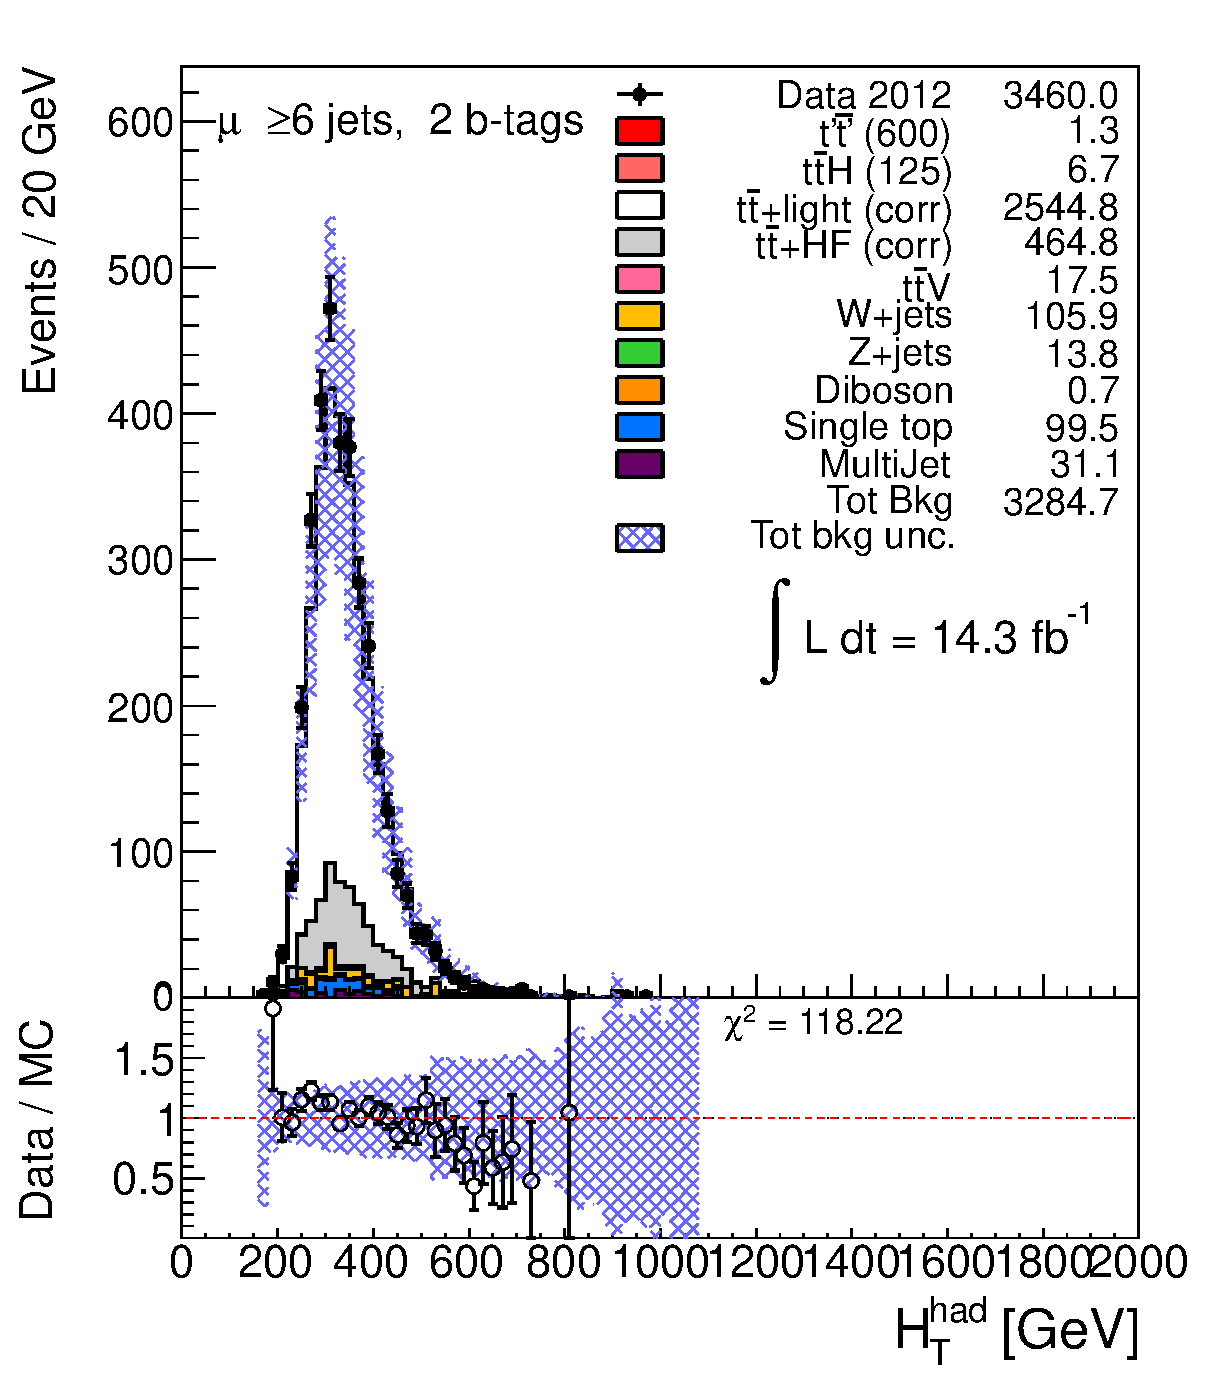
\includegraphics[width=0.3\textwidth]{appendices/figures/htx_control_unscaled/HTHad_MUON_6jetin2btagex_NOMINAL.eps}}
	\subfigure[]{
  	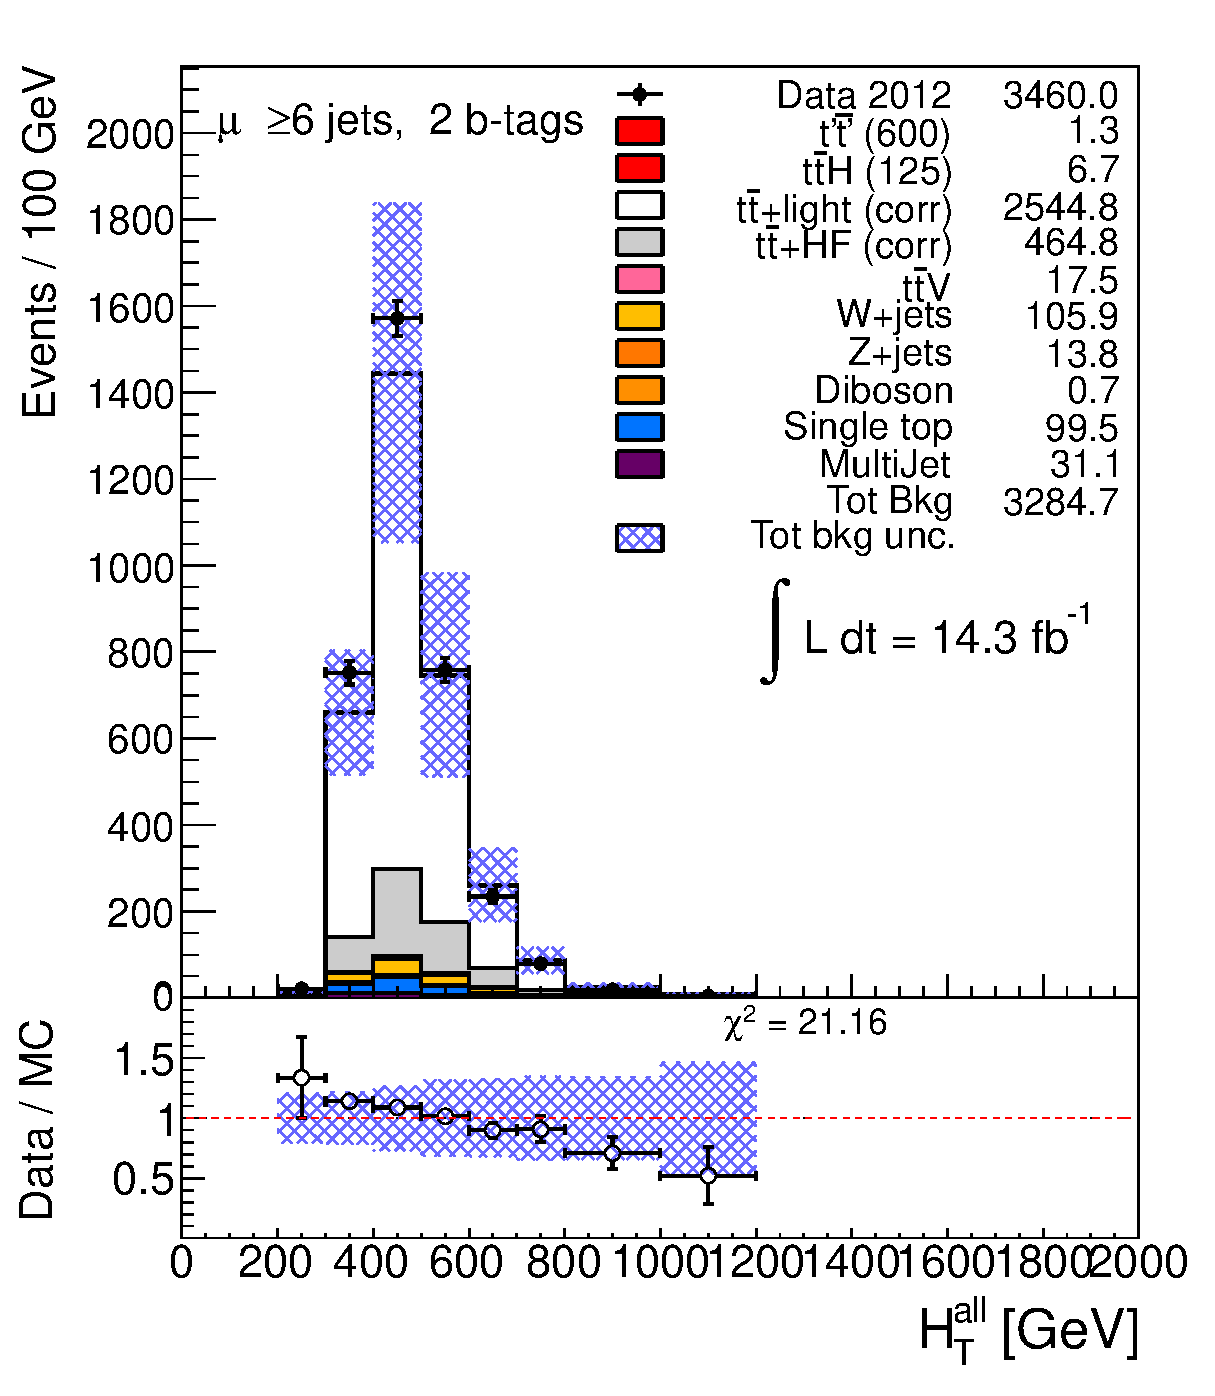
\includegraphics[width=0.3\textwidth]{appendices/figures/htx_control_unscaled/HTAll_MUON_6jetin2btagex_NOMINAL.eps}}
}\\
\hskip-2cm
\resizebox{1.5\textwidth}{!}{
	\subfigure[]{
  	\includegraphics[width=0.3\textwidth]{appendices/figures/htx_control_unscaled/LepPt_MUON_6jetin3btagex_NOMINAL.eps}}
	\subfigure[]{
  	\includegraphics[width=0.3\textwidth]{appendices/figures/htx_control_unscaled/MET_MUON_6jetin3btagex_NOMINAL.eps}}
	\subfigure[]{
  	\includegraphics[width=0.3\textwidth]{appendices/figures/htx_control_unscaled/JetPt1_MUON_6jetin3btagex_NOMINAL.eps}}
	\subfigure[]{
  	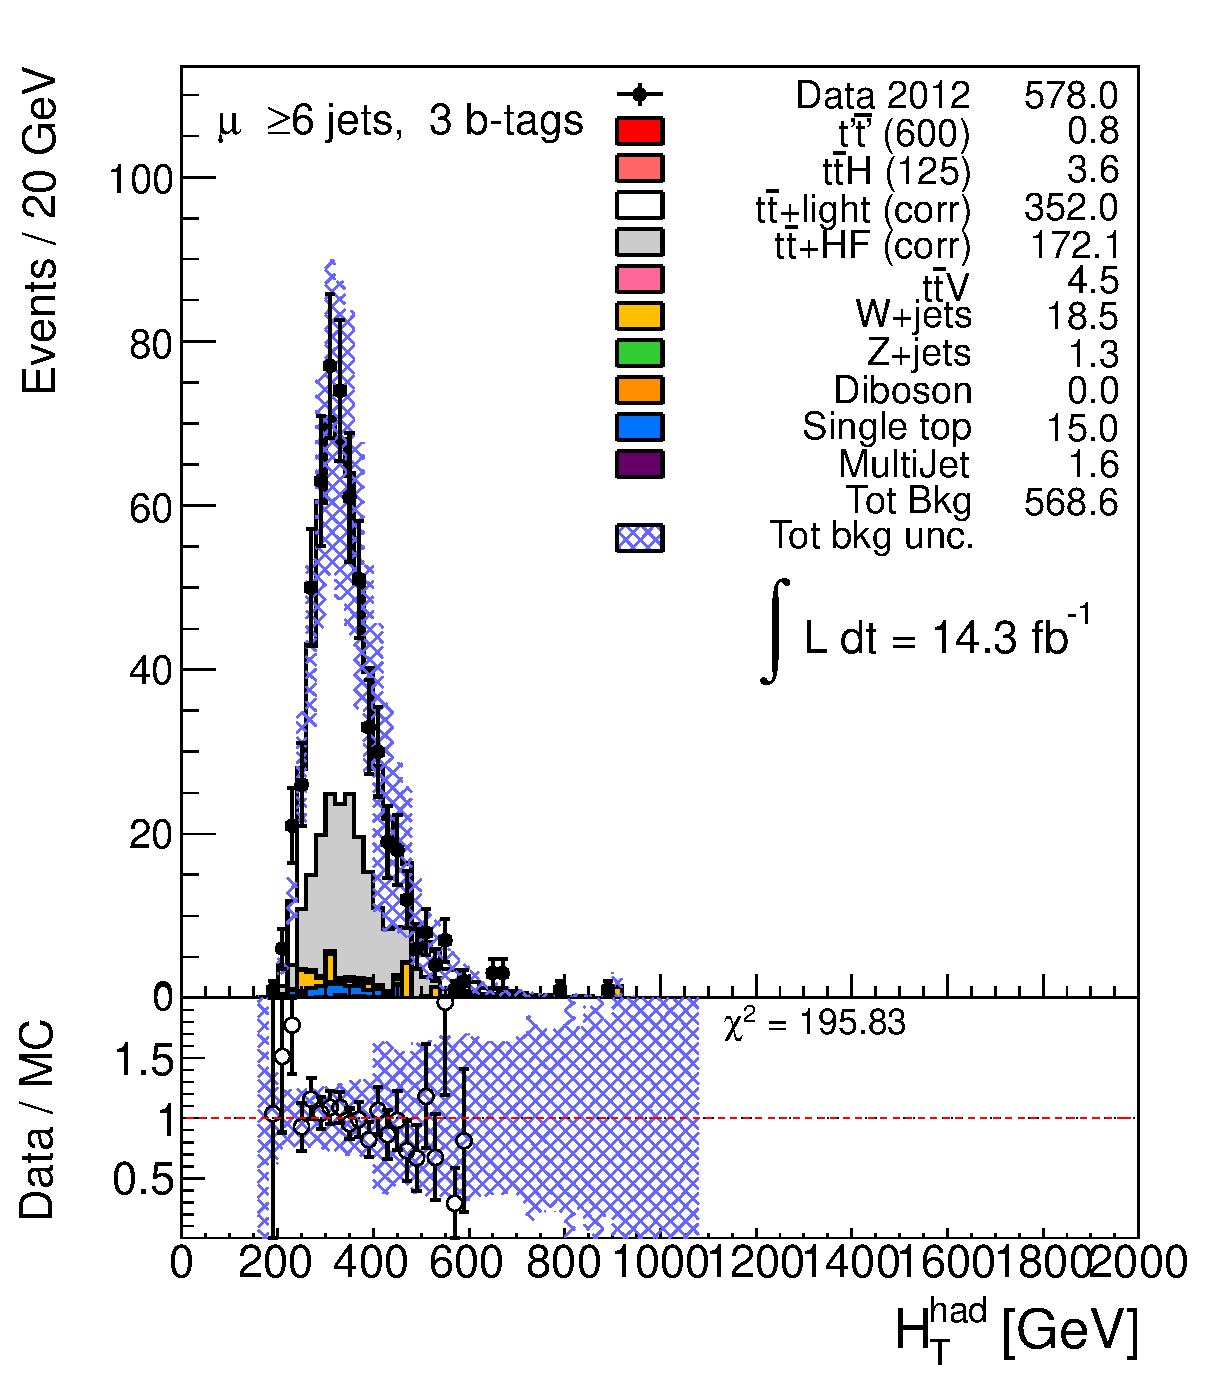
\includegraphics[width=0.3\textwidth]{appendices/figures/htx_control_unscaled/HTHad_MUON_6jetin3btagex_NOMINAL.eps}}
	\subfigure[]{
  	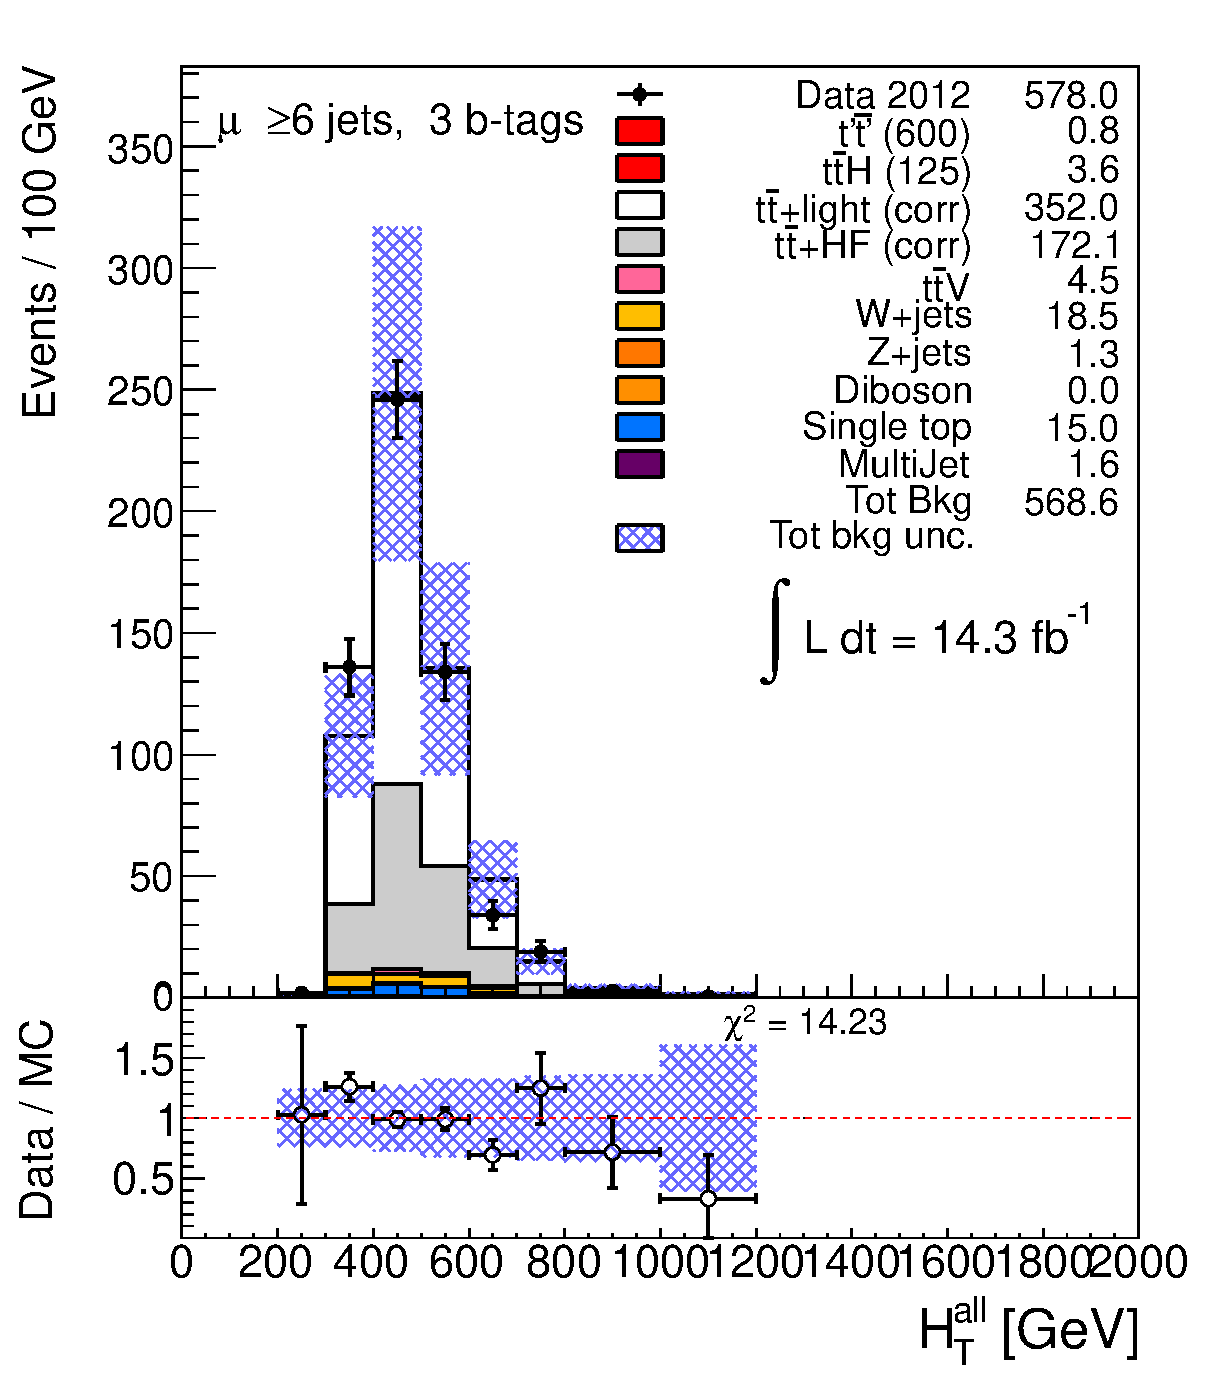
\includegraphics[width=0.3\textwidth]{appendices/figures/htx_control_unscaled/HTAll_MUON_6jetin3btagex_NOMINAL.eps}}
}\\
\hskip-2cm
\resizebox{1.5\textwidth}{!}{
	\subfigure[]{
  	\includegraphics[width=0.3\textwidth]{appendices/figures/htx_control_unscaled/LepPt_MUON_6jetin4btagin_NOMINAL.eps}}
	\subfigure[]{
  	\includegraphics[width=0.3\textwidth]{appendices/figures/htx_control_unscaled/MET_MUON_6jetin4btagin_NOMINAL.eps}}
	\subfigure[]{
  	\includegraphics[width=0.3\textwidth]{appendices/figures/htx_control_unscaled/JetPt1_MUON_6jetin4btagin_NOMINAL.eps}}
	\subfigure[]{
  	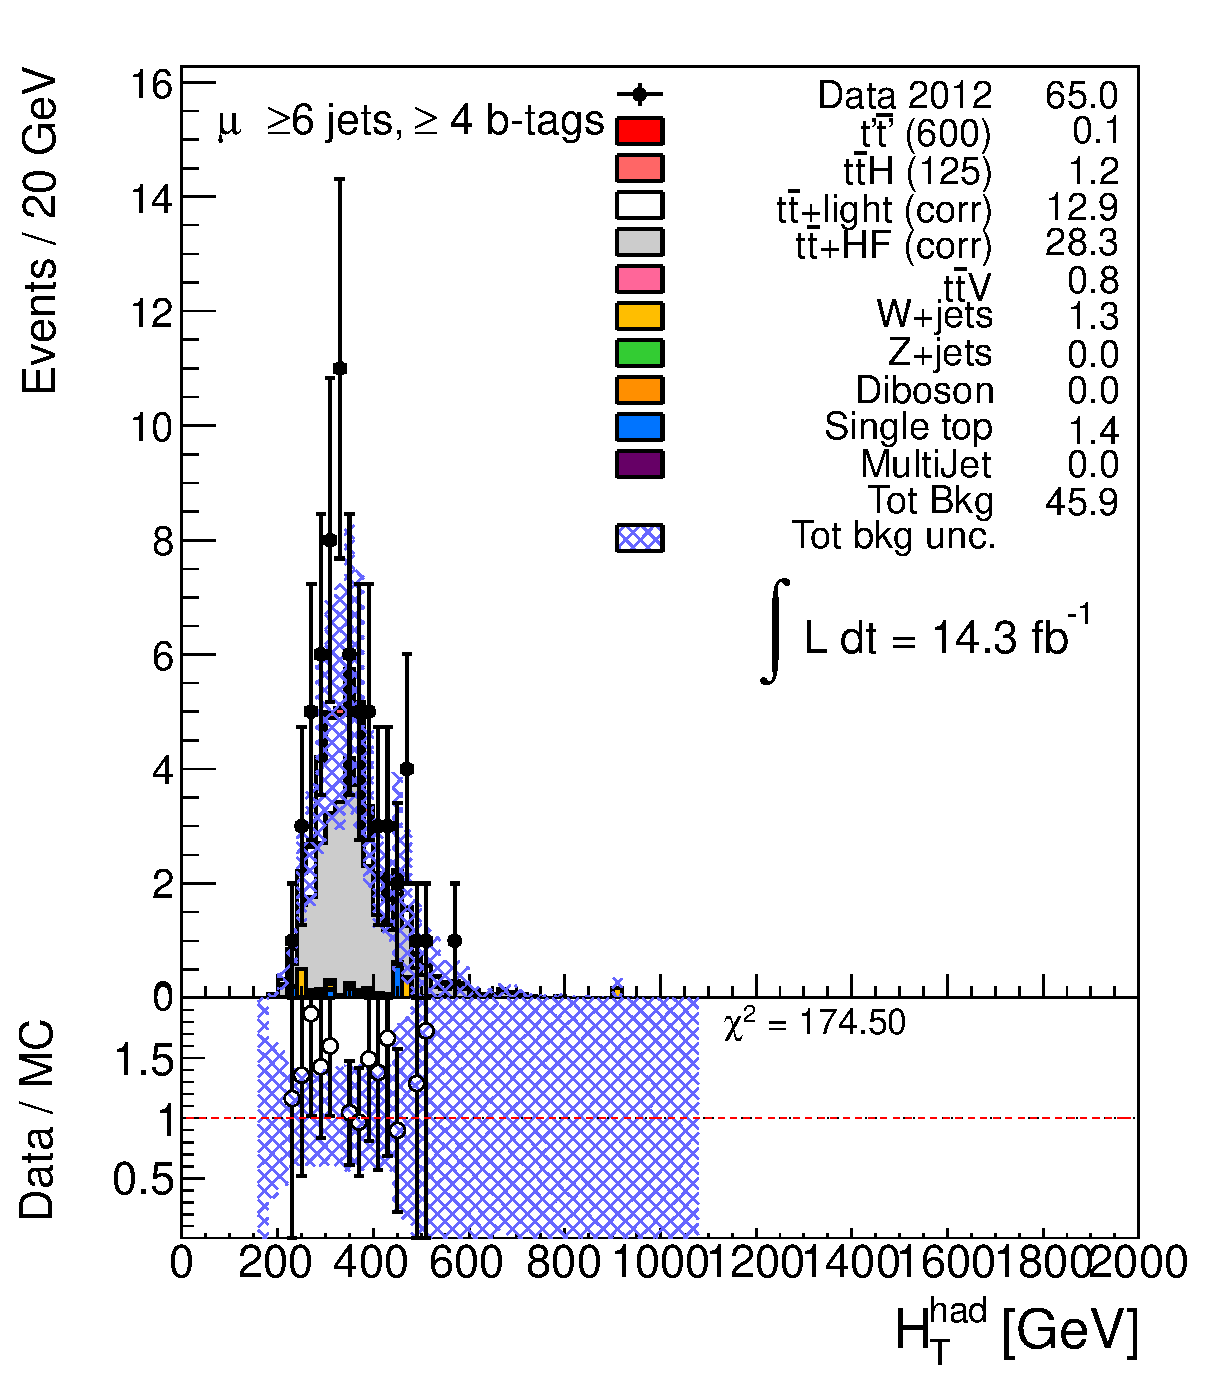
\includegraphics[width=0.3\textwidth]{appendices/figures/htx_control_unscaled/HTHad_MUON_6jetin4btagin_NOMINAL.eps}}
	\subfigure[]{
  	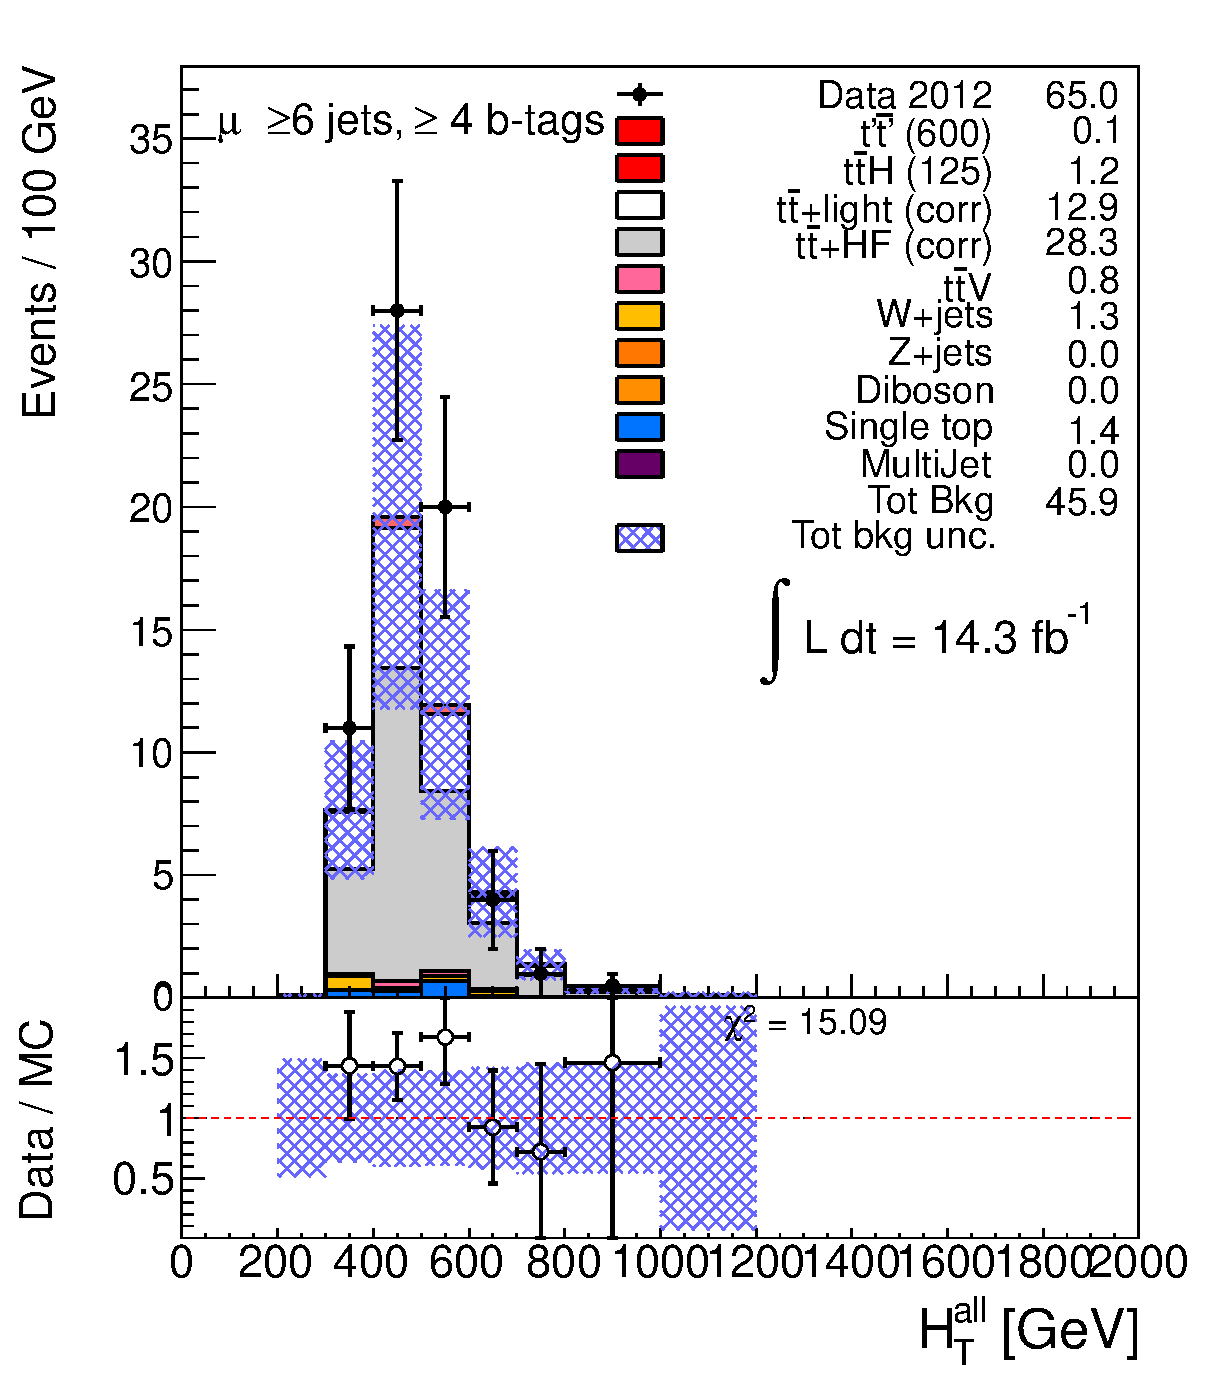
\includegraphics[width=0.3\textwidth]{appendices/figures/htx_control_unscaled/HTAll_MUON_6jetin4btagin_NOMINAL.eps}}
}
	\caption{Comparison between data and prediction in the $e$+jets channel in the blindend channels
          \chii\ (a--e), \chiii\ jets (f--j), \chiv\ jets (k--o) for a number of kinematic
          variables: from left to right, lepton $\pt$, missing transverse energy, 
          leading jet $\pt$, $\hthad$ and $\HT$. The shaded area represents the total background uncertainty.
\label{fig:selMUON_6jetin}}
\end{center}\end{figure}
\end{landscape}



